% Offline Appendix for "Same Storm, Different Boats"
%
% NOT FOR PUBLICATION — supplementary material for co-authors and replication.
% This file is not part of the journal submission. It preserves material moved
% from the Online Appendix during revision, for transparency and co-author review.
%
% Each section is self-contained and can be restored to appendix.tex by
% uncommenting the corresponding stub in that file.
%
% This file compiles standalone with tectonic for verification.

\documentclass[preprint,12pt,authoryear]{elsarticle}

\usepackage[utf8]{inputenc}
\usepackage[T1]{fontenc}
\usepackage{amsmath,amssymb}
\usepackage{graphicx}
\usepackage{booktabs}
\usepackage[colorlinks=true, allcolors=blue]{hyperref}
\usepackage{natbib}

\graphicspath{{../figures/}}

\begin{document}

\begin{frontmatter}
\title{Offline Appendix: Same Storm, Different Boats: Generative AI and the Age Gradient in Hiring}
\author{Lodefalk, L\"{o}thman, Koch, and Engberg}
\end{frontmatter}

\setcounter{section}{0}
\renewcommand{\thesection}{OA\arabic{section}}
\renewcommand{\thetable}{OA\arabic{table}}
\renewcommand{\thefigure}{OA\arabic{figure}}

\noindent This document contains supplementary material moved from the Online Appendix during revision. All material is preserved for transparency and is available in the project repository at \url{https://github.com/Magnus-L/canaries-sweden}. Sections can be restored to the Online Appendix by uncommenting the corresponding stubs in \texttt{appendix.tex}.


% ══════════════════════════════════════════════════════════════════════════════
%   OA1: Stock market composition (formerly Online Appendix, Part II)
% ══════════════════════════════════════════════════════════════════════════════

\section{Stock market composition: Sweden vs the US}

The ``scary chart'' narrative implicitly assumes that stock market gains reflect AI-driven revaluation. This is plausible for the US, where AI-adjacent firms (the ``Magnificent~7'': Alphabet, Amazon, Apple, Meta, Microsoft, Nvidia, Tesla) accounted for the majority of S\&P~500 gains in 2023--2025. The Swedish OMXS30, however, is dominated by industrials (Atlas~Copco, Volvo, Sandvik), banks (SEB, Handelsbanken, Swedbank), and telecommunications (Ericsson), with limited direct AI exposure.

Figure~\ref{fig:stock_comparison} indexes the OMXS30, S\&P~500, and Nasdaq Composite to February 2020~=~100. By early 2026, the Nasdaq -- the most AI-weighted major index -- reached approximately 243, the S\&P~500 approximately 210, and the OMXS30 approximately 171. The 72-point gap between Nasdaq and OMXS30 opened primarily after the ChatGPT launch, consistent with the Nasdaq reflecting AI expectations while the OMXS30 reflects export earnings (amplified by a weak krona) and banking margins. The Swedish stock-posting divergence is therefore better characterised as a coincidence of distinct macroeconomic forces -- monetary tightening depressing postings, global equity sentiment and krona weakness lifting share prices -- rather than AI simultaneously boosting equity values and destroying jobs.

\begin{figure}[htbp]
\centering
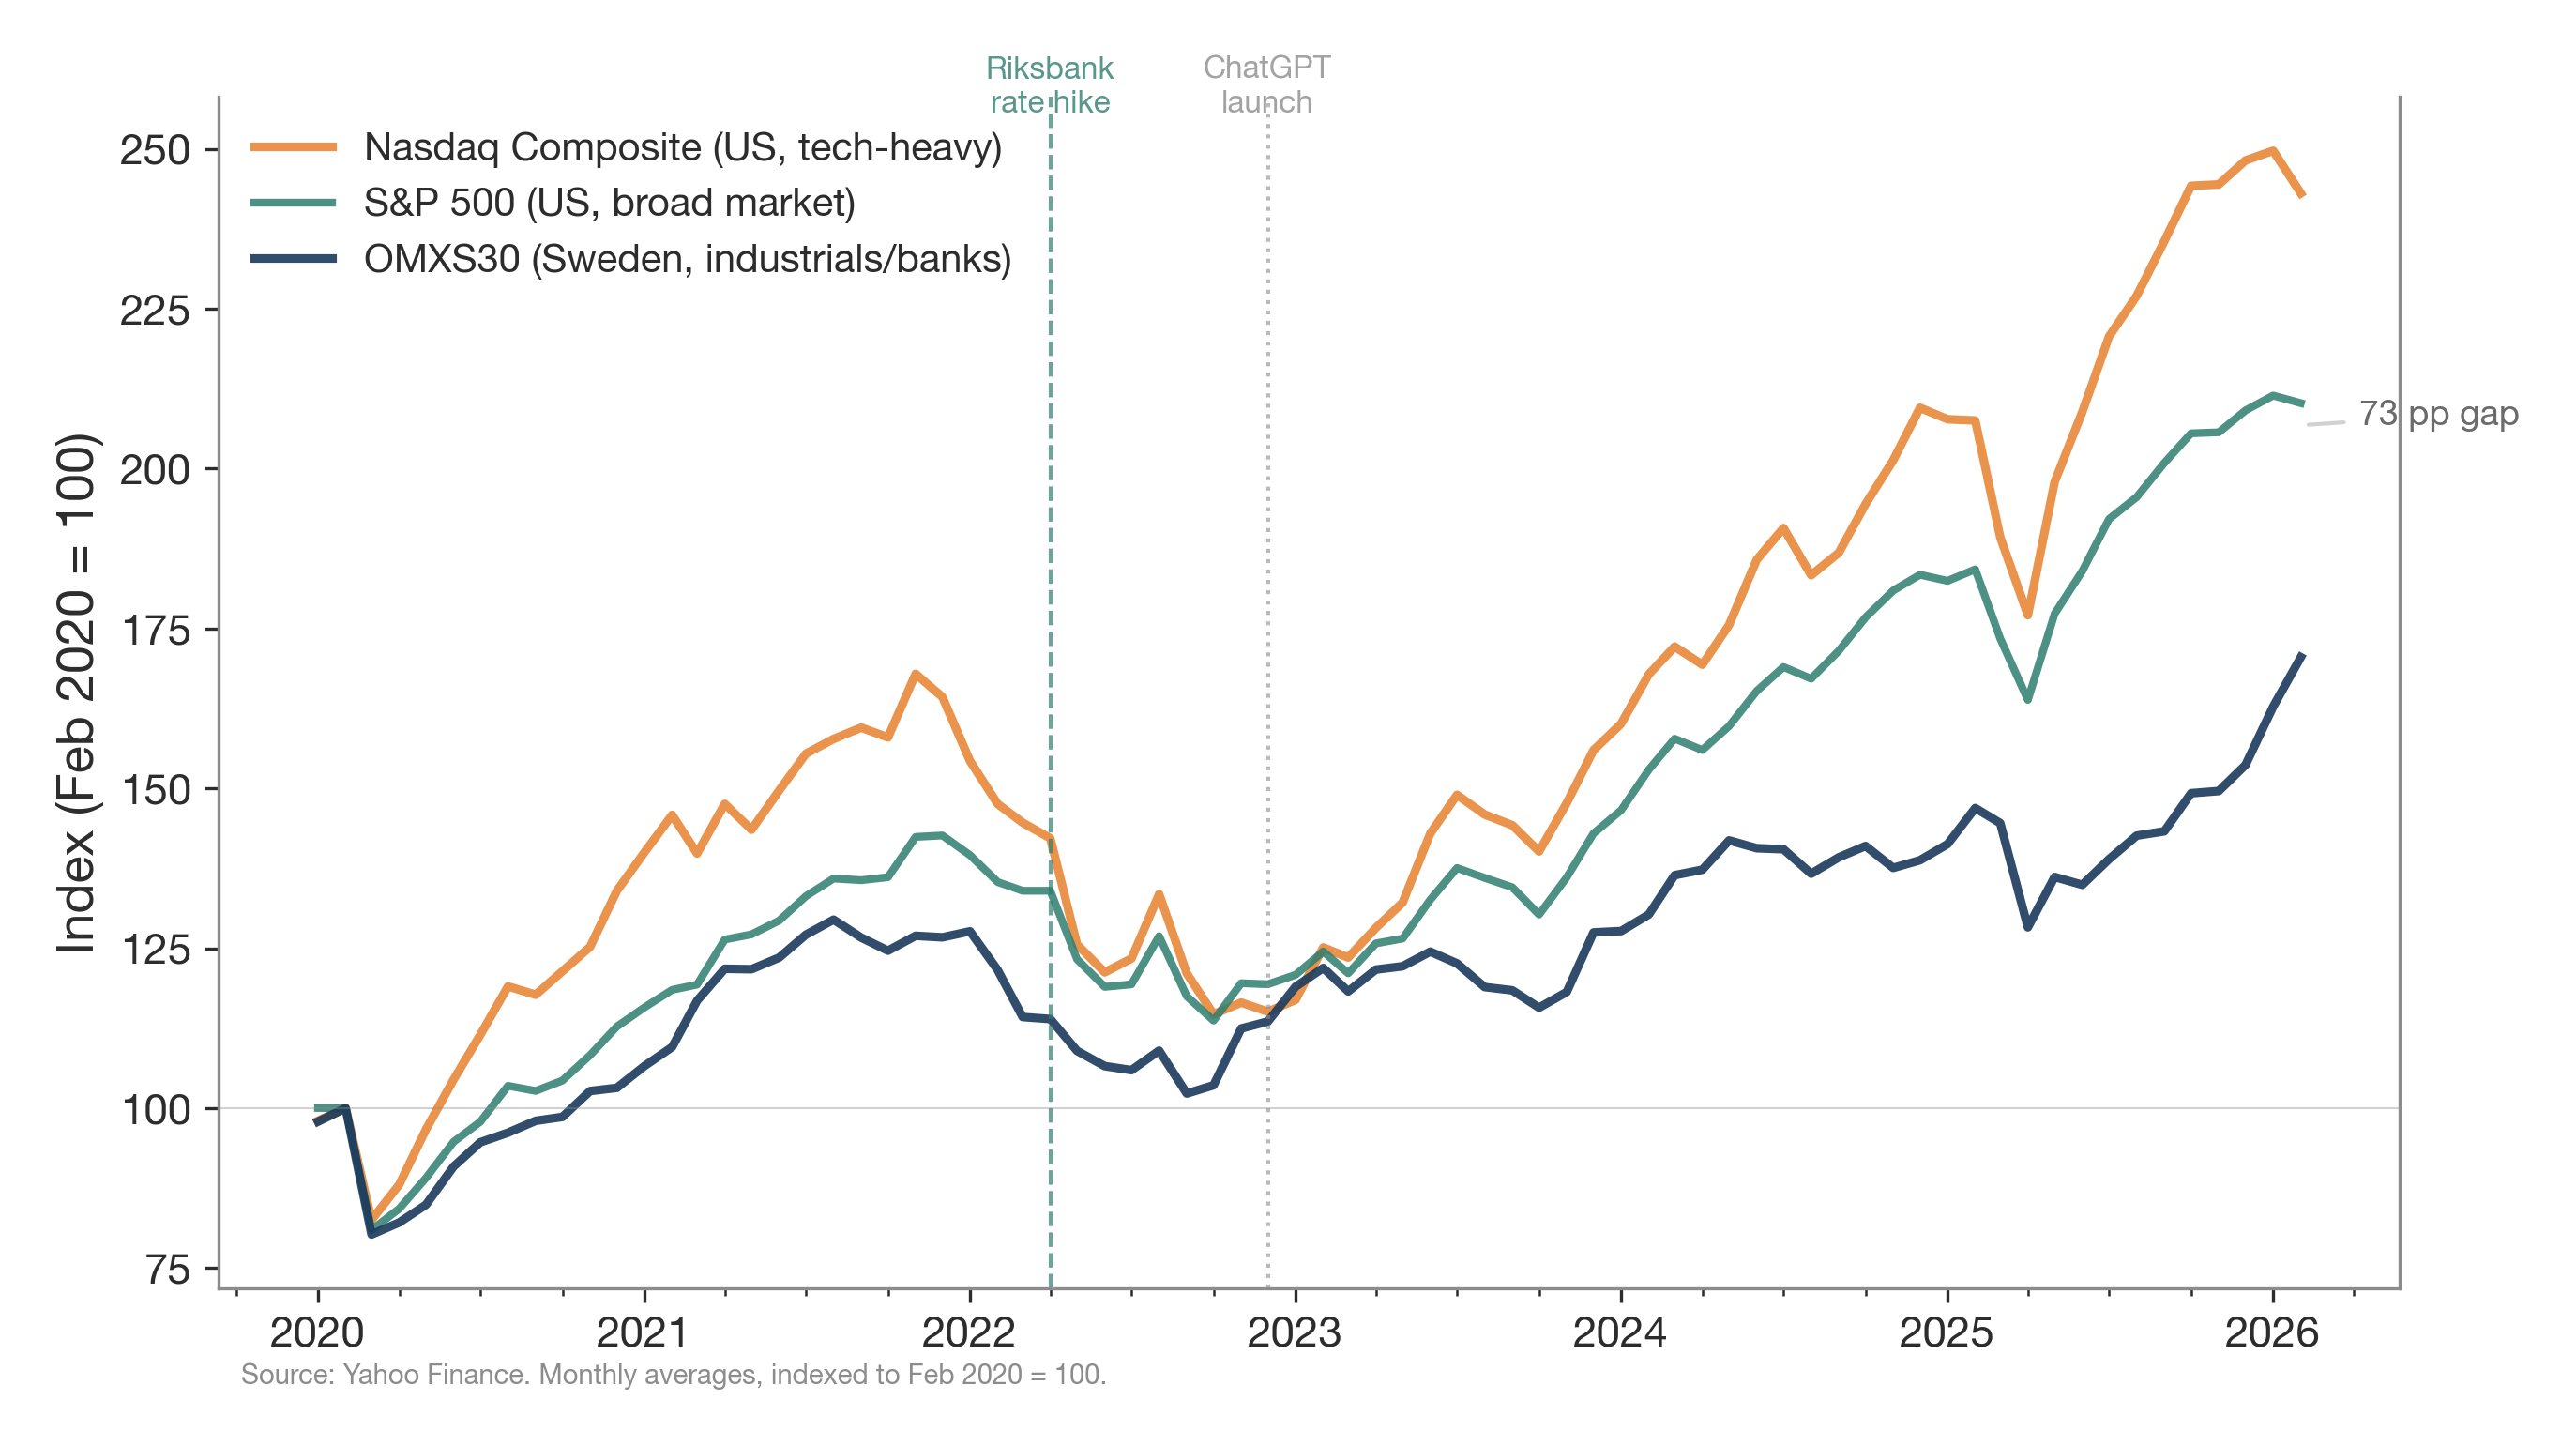
\includegraphics[width=\textwidth]{figA12_stock_market_comparison.png}
\caption{Stock market indices, 2020--2026: OMXS30 (Sweden), S\&P~500 (US, broad), and Nasdaq Composite (US, tech-heavy). Monthly averages, indexed to February 2020 = 100. Vertical lines mark the Riksbank's first rate hike (April 2022) and ChatGPT launch (November 2022). The gap between Nasdaq and OMXS30 widens after ChatGPT, consistent with US AI-driven equity revaluation absent in the Swedish index.}
\label{fig:stock_comparison}
\end{figure}


% ══════════════════════════════════════════════════════════════════════════════
%   OA2: Posting gap Q4 vs Q1 (formerly Online Appendix, Part II)
% ══════════════════════════════════════════════════════════════════════════════

\section{Posting gap: top vs bottom quartile}

Figure~\ref{fig:exposure_gap} plots the difference in posting indices between Q4 (highest genAI exposure) and Q1 (lowest) over time. The gap fluctuates around zero throughout the sample period, including after the ChatGPT launch. There is no visible widening of the gap following November 2022, as would be expected if AI were differentially reducing postings in exposed occupations.

\begin{figure}[htbp]
\centering
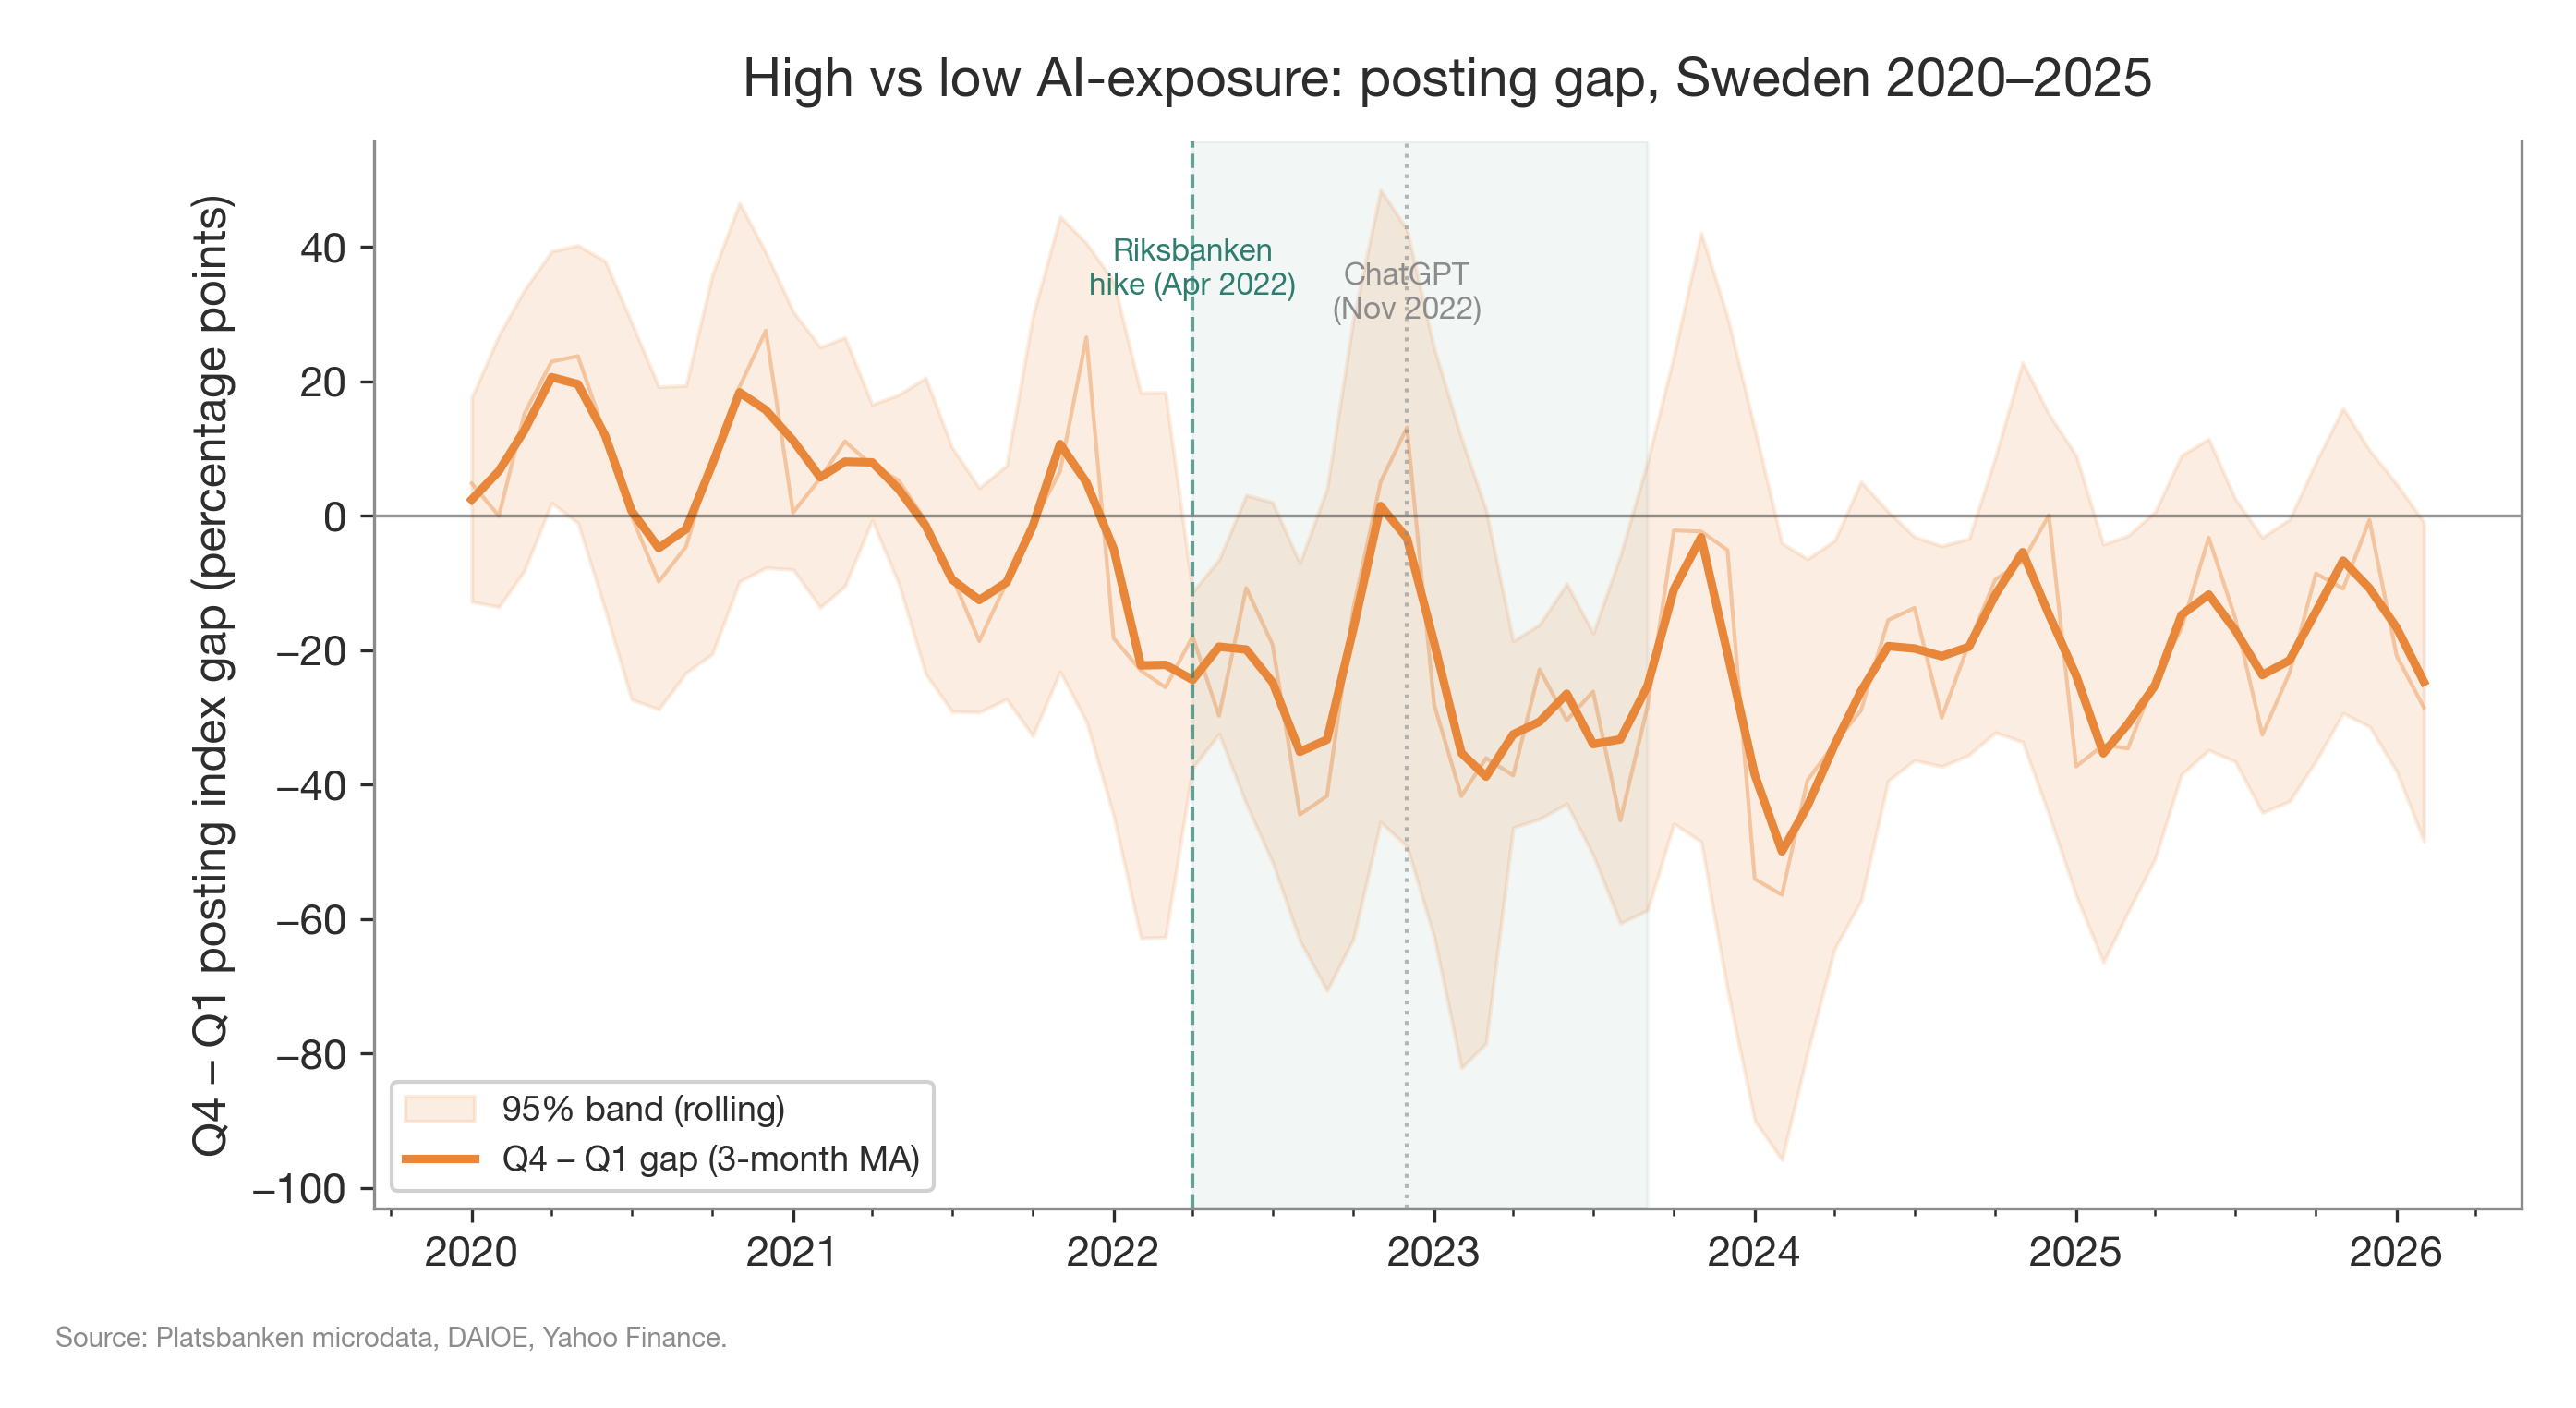
\includegraphics[width=\textwidth]{fig2_exposure_gap.png}
\caption{Posting index gap between Q4 (highest genAI exposure) and Q1 (lowest), with 3-month moving average and 95\% confidence band. No systematic widening after ChatGPT.}
\label{fig:exposure_gap}
\end{figure}


% ══════════════════════════════════════════════════════════════════════════════
%   OA3: Quarterly posting event study (formerly Online Appendix, Part II)
% ══════════════════════════════════════════════════════════════════════════════

\section{Event study (quarterly)}

Figure~\ref{fig:eventstudy_q} aggregates the monthly event study to quarterly frequency, reducing noise but preserving the key patterns.

\begin{figure}[htbp]
\centering
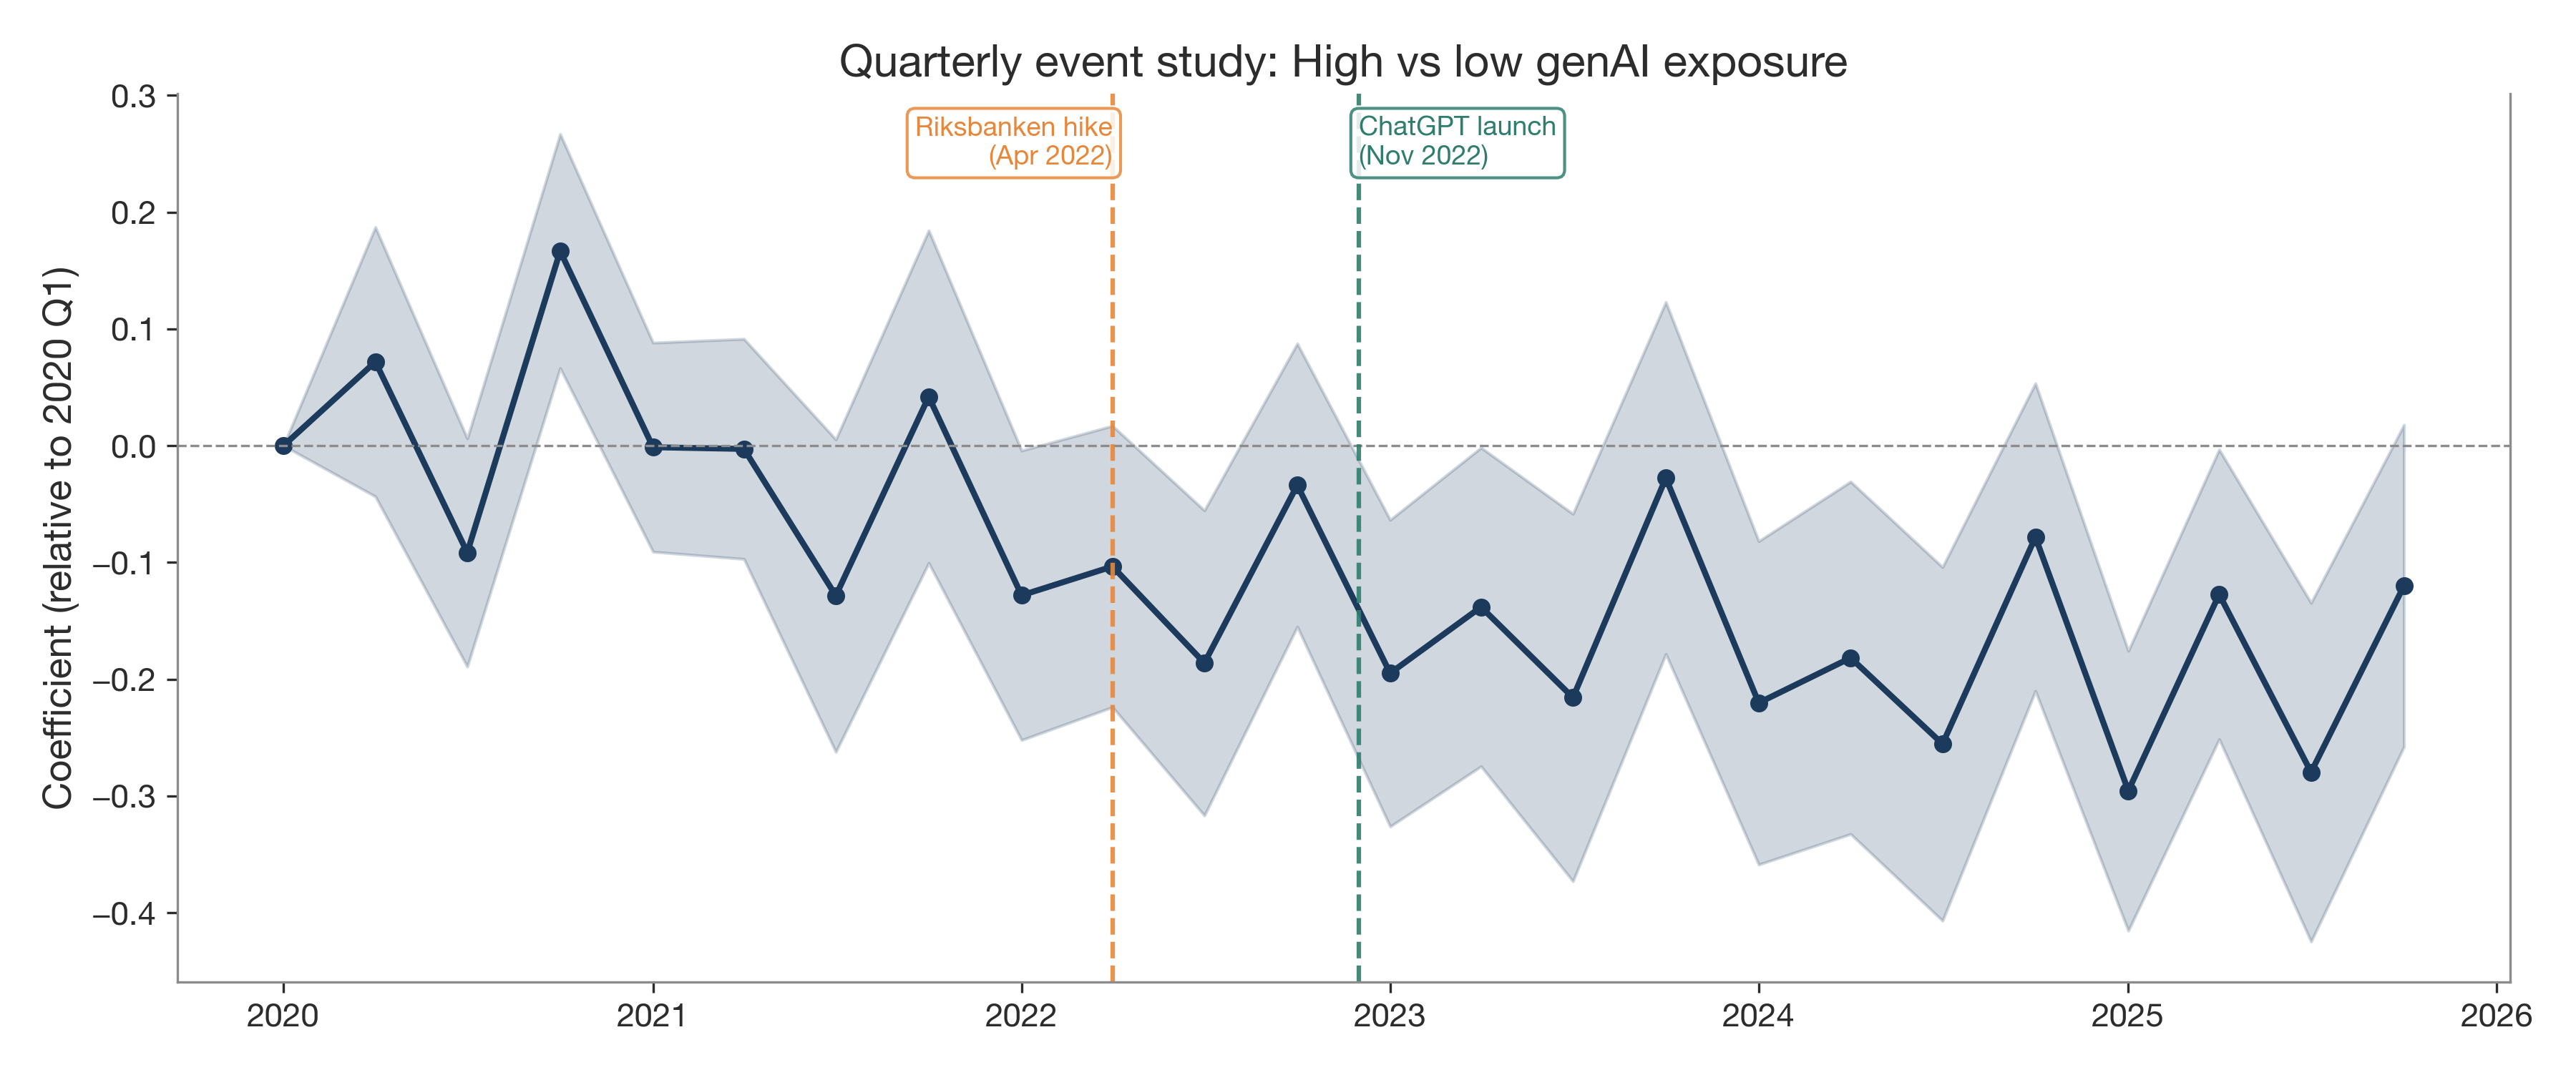
\includegraphics[width=\textwidth]{figA5_event_study_quarterly.png}
\caption{Quarterly event study: DiD coefficients for high vs low genAI exposure occupations (reference: 2020~Q1). Shaded area shows 95\% confidence interval. Aggregating to quarters reduces monthly noise but pre-period differentials remain jointly significant ($\chi^2_{8} = 52.8$, $p < 0.01$), reflecting differential macro sensitivity.}
\label{fig:eventstudy_q}
\end{figure}


% ══════════════════════════════════════════════════════════════════════════════
%   OA4: Half-year posting event study (formerly Online Appendix, Part II)
% ══════════════════════════════════════════════════════════════════════════════

\section{Half-year posting event study}

Figure~\ref{fig:halfyear_es} aggregates the event study to half-year periods, with 2022H1 (pre-Riksbank hike) as the reference. Pre-period coefficients are positive and significant, indicating that high-AI-exposure occupations had relatively more postings before the treatment period. After the reference period, coefficients drift negative: the 2023H1 coefficient is marginally significant ($-0.066$, $p = 0.08$), while 2025H1 and 2025H2 reach marginal significance ($-0.094$ and $-0.099$, both $p < 0.10$). The 2026H1 estimate ($-0.412$, $p < 0.01$) is based on only two months and should be interpreted cautiously. The gradual negative drift, rather than a sharp break at the ChatGPT launch (2022H2), is consistent with the main finding that the posting decline is driven by macroeconomic factors with at most a small additional AI component.

\begin{figure}[htbp]
\centering
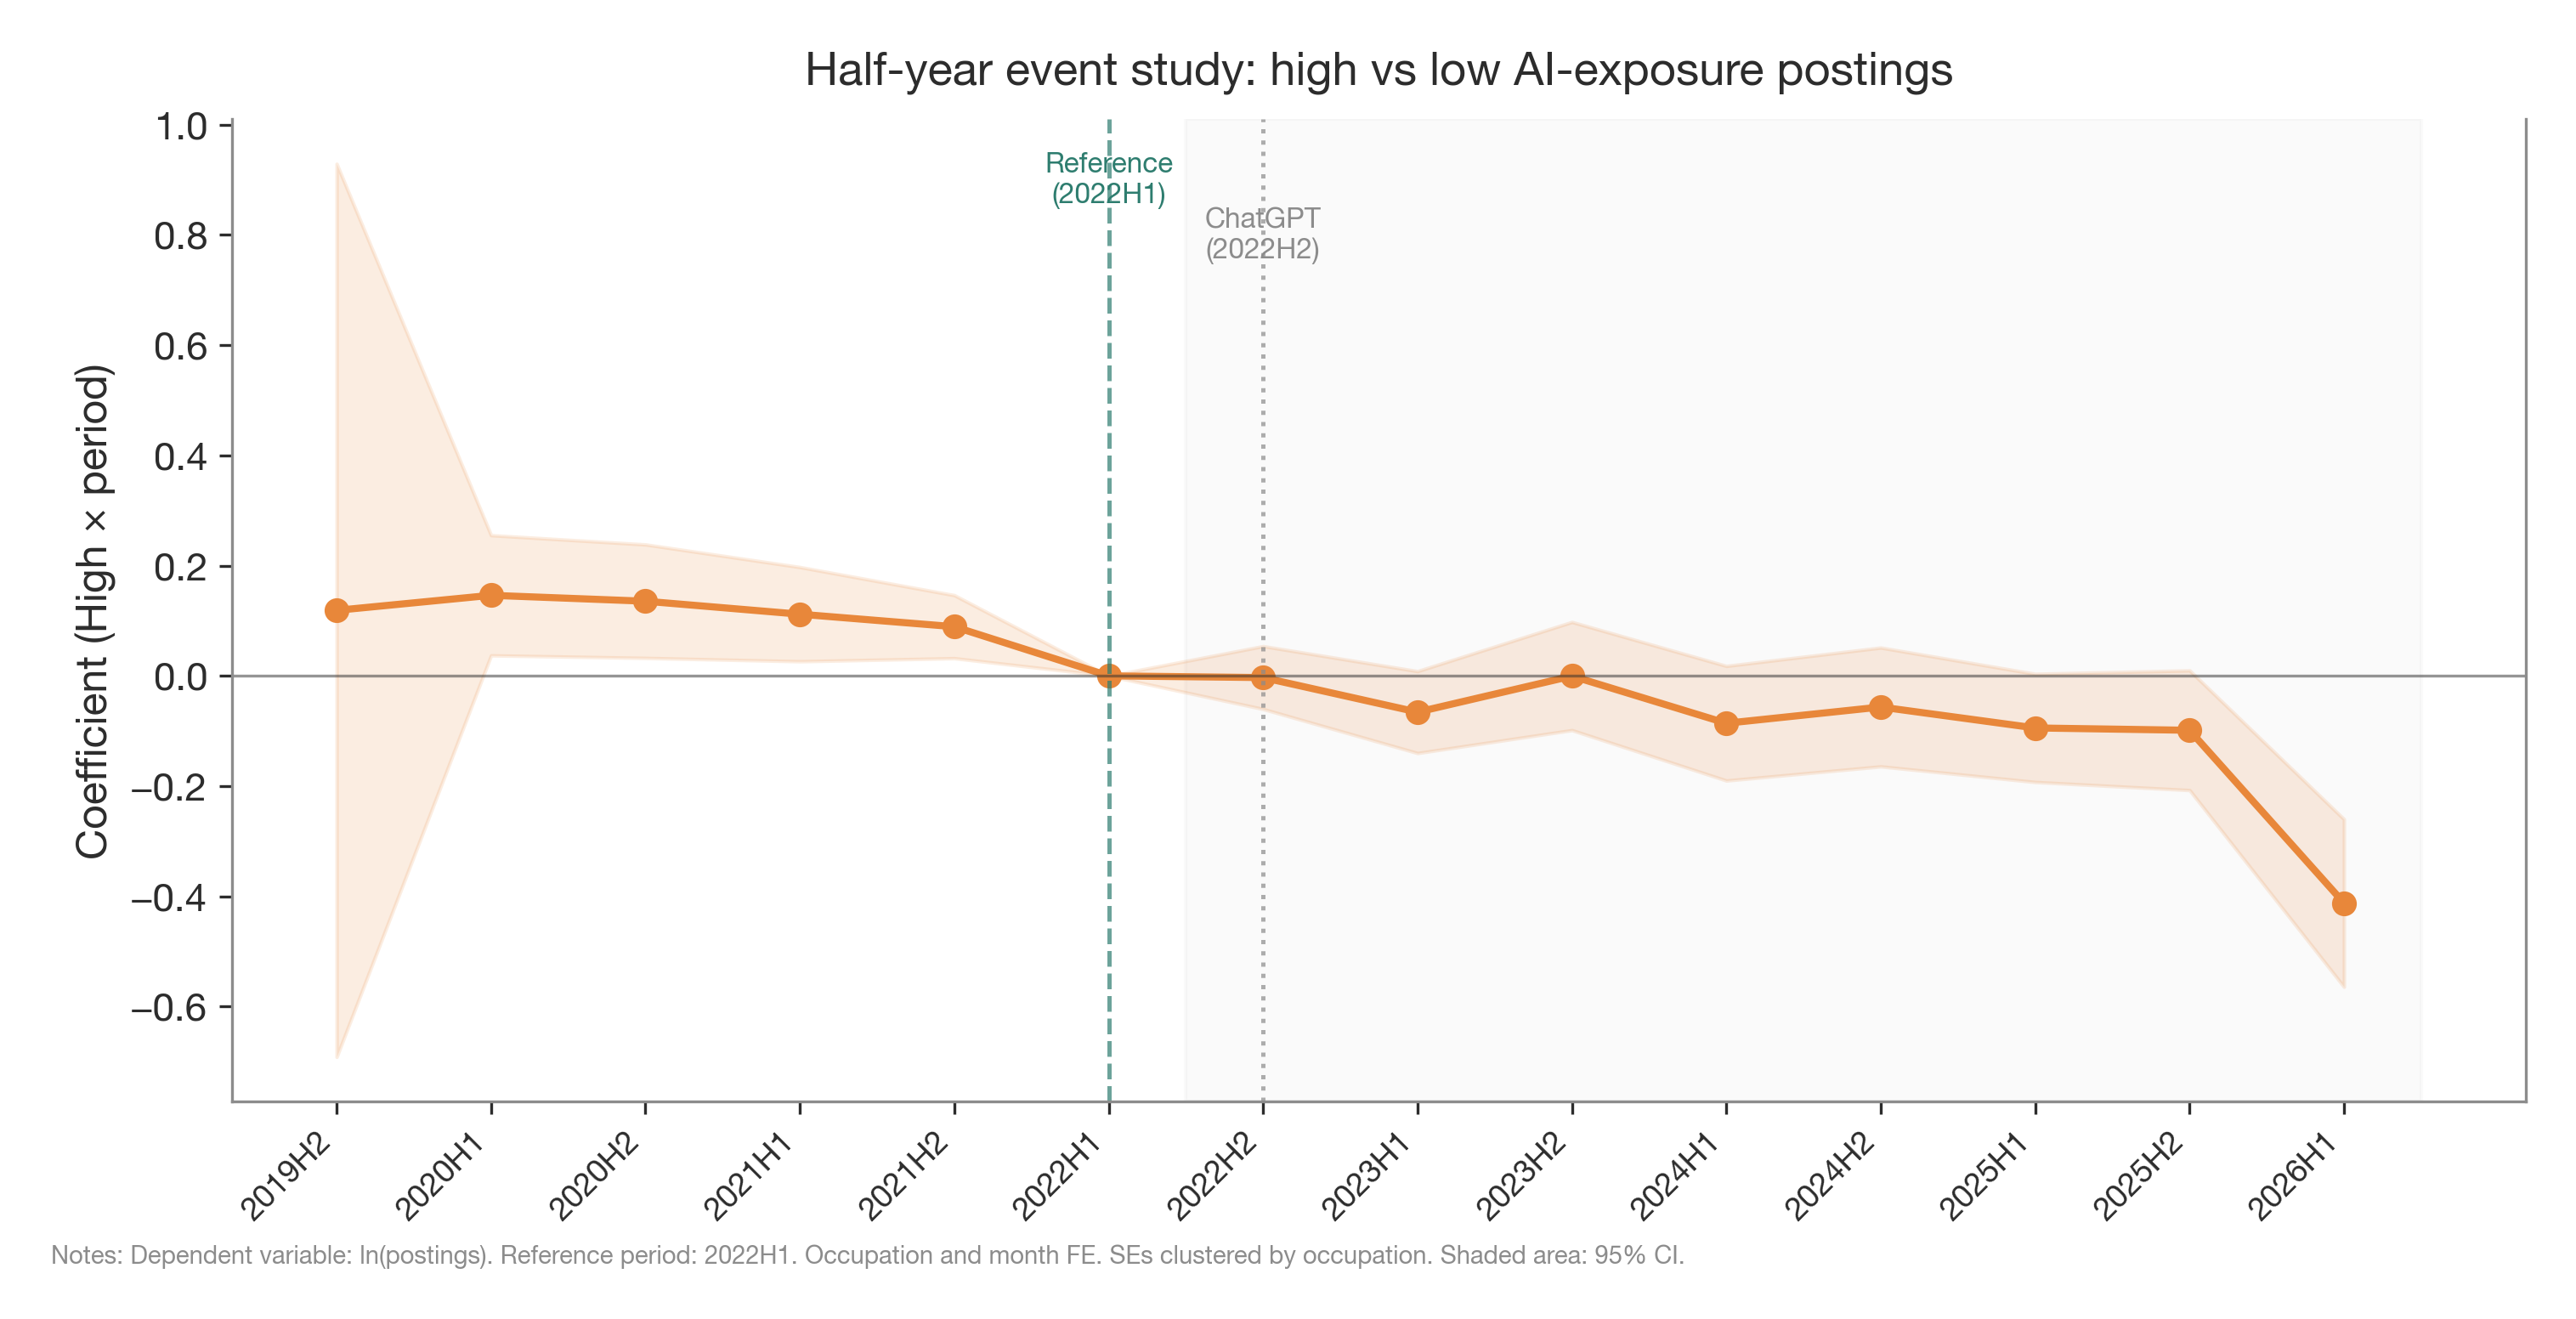
\includegraphics[width=\textwidth]{figA11_halfyear_event_study.png}
\caption{Half-year event study: coefficients on High $\times$ half-year period interactions (reference: 2022H1). Occupation and month fixed effects; standard errors clustered by occupation. Shaded area: 95\% confidence interval. The gradual negative drift after 2022 is consistent with broad-based macro effects rather than a discrete AI shock.}
\label{fig:halfyear_es}
\end{figure}


% ══════════════════════════════════════════════════════════════════════════════
%   OA5: YREG annual employment data (formerly Online Appendix, Part III)
% ══════════════════════════════════════════════════════════════════════════════

\section{Annual employment by age group and AI exposure (YREG)}

\citet{brynjolfsson2025canaries} find that young US workers in AI-exposed occupations experienced disproportionate employment declines, ``canaries in the coal mine.'' Our posting-based analysis cannot test this age-specific hypothesis directly. As a first check, we use publicly available register data from SCB (Yrkesregistret, table YREG54BAS) providing annual employment counts by SSYK~4-digit occupation and age group for 2020--2024. These annual data show no visible divergence between young workers in high- vs low-AI-exposure occupations after ChatGPT, but three caveats limit their informativeness: (i)~SCB changed the underlying register from RAMS to BAS from reference year 2022, introducing a methodological break at our treatment timing; (ii)~the 2020 pandemic trough as base year inflates all growth rates; (iii)~with only five annual observations, statistical power is limited.

\begin{figure}[htbp]
\centering
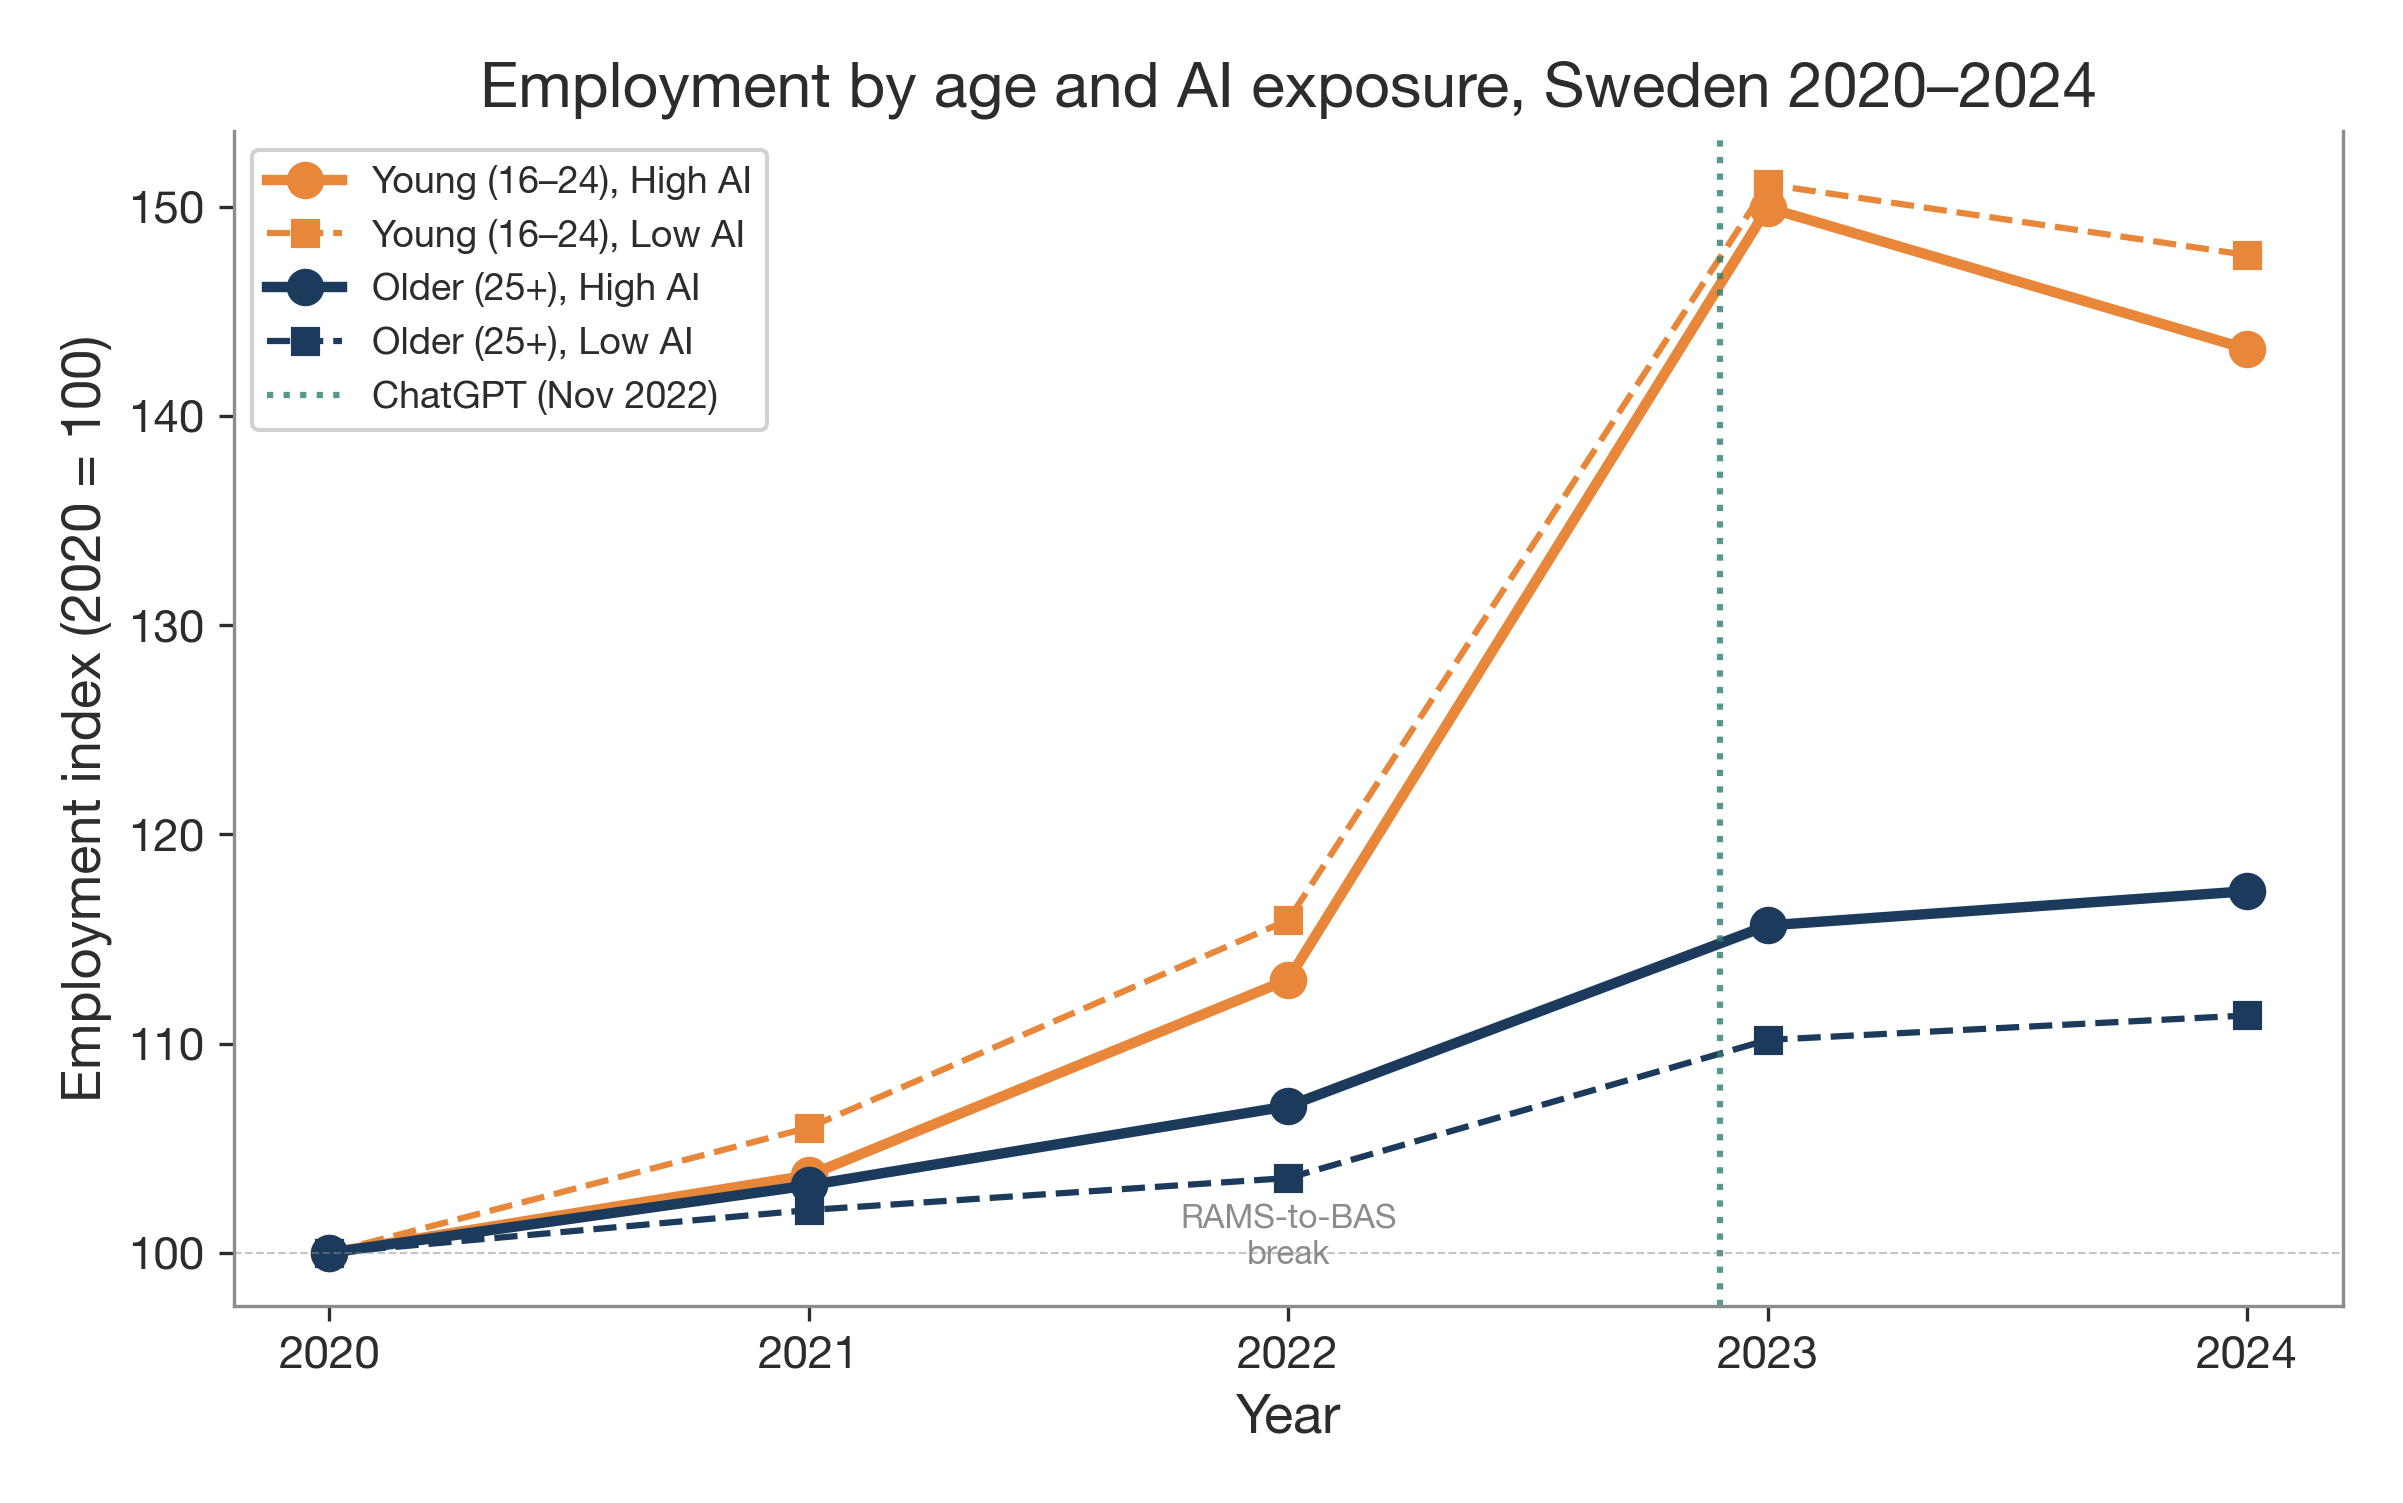
\includegraphics[width=\textwidth]{figA7_canaries_employment.png}
\caption{Employment by age group and AI exposure, Sweden 2020--2024 (2020 = 100). Data: SCB Yrkesregistret (YREG54BAS). Young = 16--24 years; High AI = top quartile of DAIOE genAI exposure. The dotted line marks ChatGPT launch (November 2022). Note: methodological break (RAMS to BAS) at 2022.}
\label{fig:canaries_emp}
\end{figure}


% ══════════════════════════════════════════════════════════════════════════════
%   OA6: GenAI capability timeline (formerly Online Appendix, Part III)
% ══════════════════════════════════════════════════════════════════════════════

\section{GenAI capability timeline}

The divergence between young workers in high- and low-AI-exposure occupations visible in Figure~2 of the main paper does not follow a single break but appears to deepen in stages. A factual timeline of major generative AI releases helps contextualise these patterns. ChatGPT launched on November~30, 2022; GPT-4 followed on March~14, 2023, marking the first model widely regarded as highly capable across professional tasks. Enterprise deployment accelerated in the second half of 2023: ChatGPT Enterprise launched in August~2023 and Microsoft~365 Copilot became generally available in November~2023. A second capability wave arrived in mid-2024 with GPT-4o (May~2024) and Claude~3.5 Sonnet (June~2024), both offering substantially improved coding and analytical capabilities at lower cost. Reasoning and agentic models emerged from September~2024 (OpenAI~o1, Claude computer use), followed by open-source reasoning models (DeepSeek~R1, January~2025).

Two acceleration points in the young-high-AI trajectory roughly coincide with these waves. The initial divergence from the young-low-AI group emerges in early-to-mid 2023, following GPT-4 and early enterprise experimentation. A steeper decline begins in late 2024, coinciding with the deployment of agentic and reasoning models that automate more complex task sequences. These timing correspondences are suggestive, not causal: adoption lags between model release and workplace impact are uncertain, and macroeconomic conditions also shifted in these periods. Nevertheless, the staged pattern is more consistent with cumulative technological displacement than with a single discrete shock.


% ══════════════════════════════════════════════════════════════════════════════
%   OA7: Additional event study figures (ages 31-34, 35-40, 50+)
% ══════════════════════════════════════════════════════════════════════════════

\section{Additional event study figures}

The Online Appendix presents event studies (with employer$\times$quartile and employer$\times$month fixed effects) for the three most informative age groups: 22--25, 26--30, and 41--49. The remaining age groups are shown below for completeness. All three exhibit significant pre-trends, limiting their interpretability as standalone tests of parallel trends, but the post-treatment patterns are consistent with the main DiD estimates.

\begin{figure}[htbp]
\centering
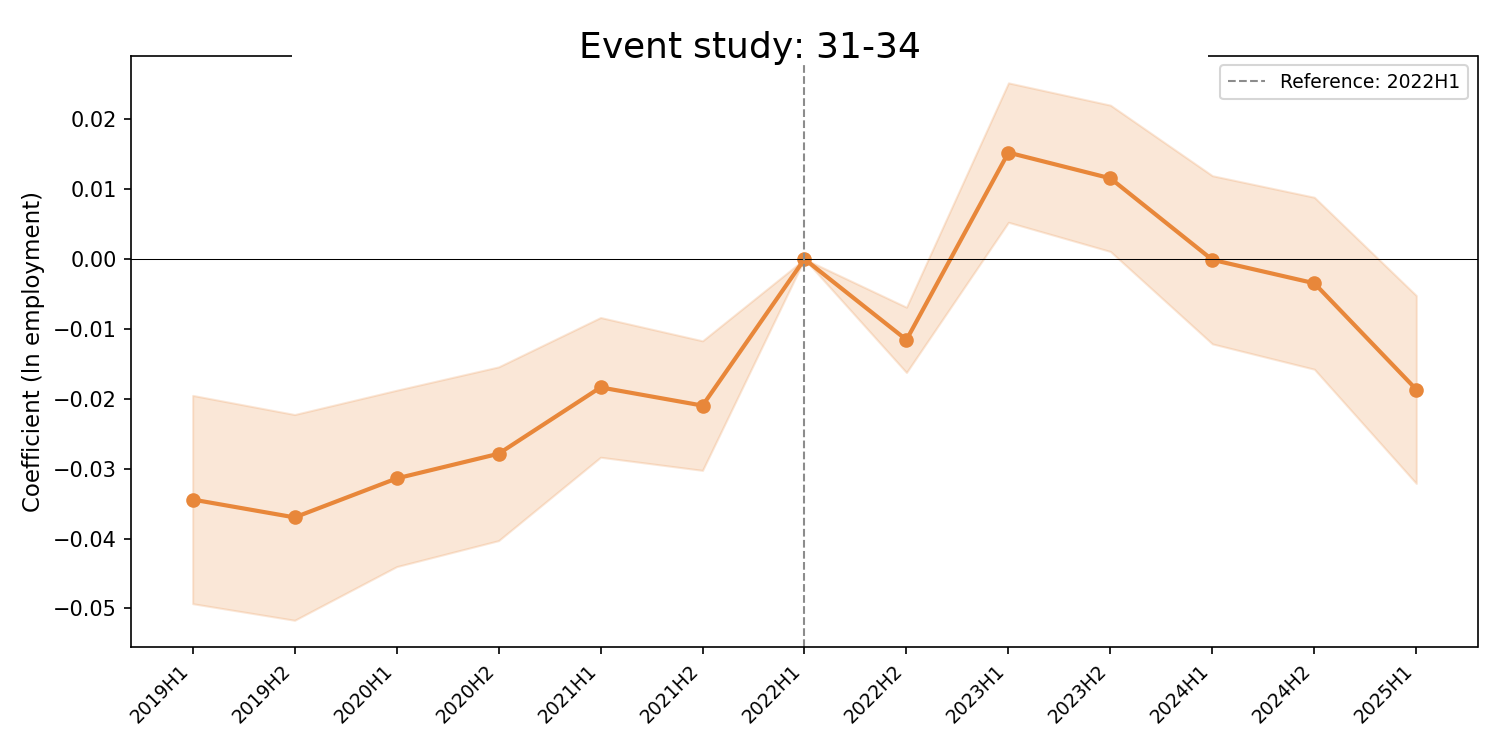
\includegraphics[width=\textwidth]{figA_es_31to34_corrected.png}
\caption{Half-year event study: ages 31--34. Employer$\times$quartile and employer$\times$month fixed effects (reference: 2022H1). Significant pre-trends ($\chi^2(6) = 120.4$, $p < 0.001$). Post-treatment coefficients close to zero, consistent with the small DiD estimate for this age group.}
\label{fig:es_31to34}
\end{figure}

\begin{figure}[htbp]
\centering
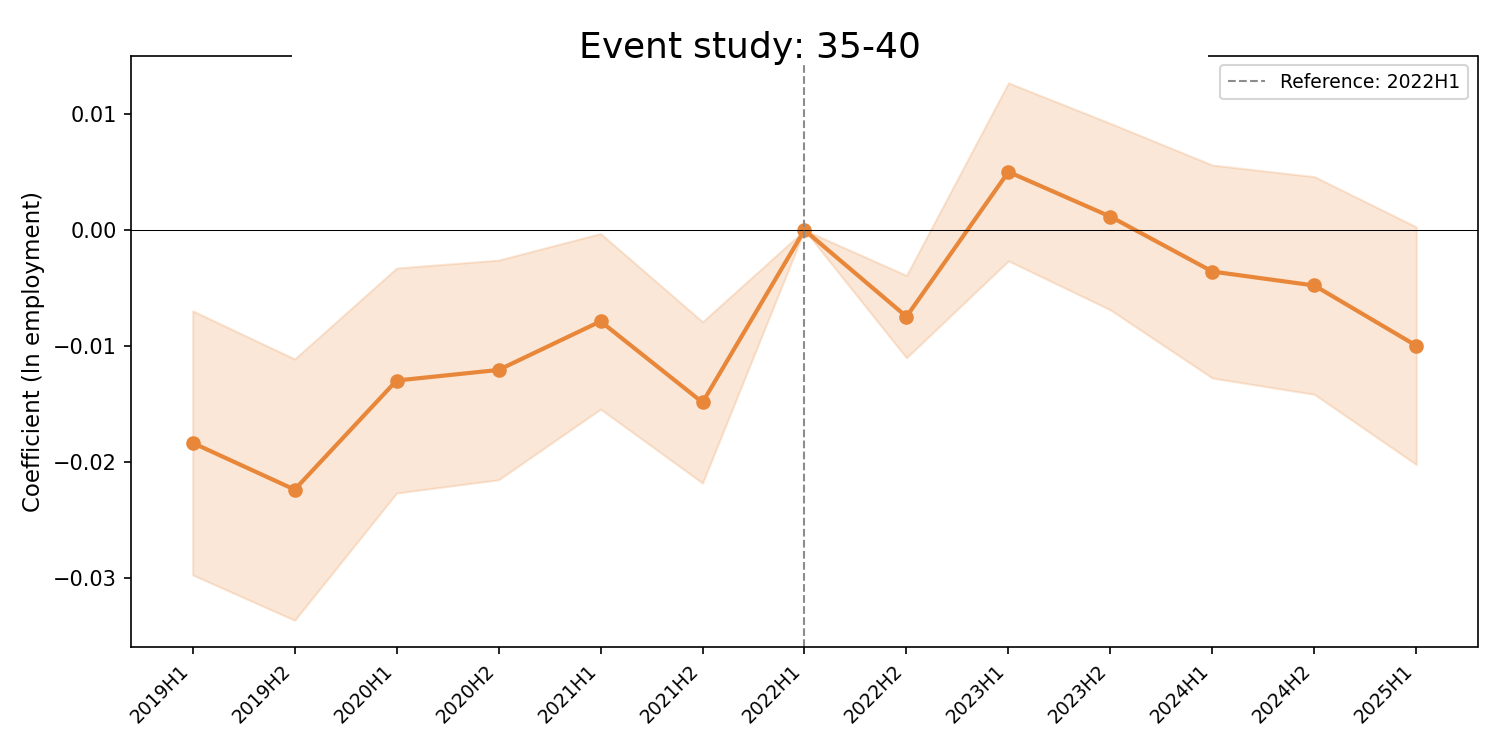
\includegraphics[width=\textwidth]{figA_es_35to40_corrected.png}
\caption{Half-year event study: ages 35--40. Employer$\times$quartile and employer$\times$month fixed effects (reference: 2022H1). Significant pre-trends ($\chi^2(6) = 59.9$, $p < 0.001$). Post-treatment coefficients close to zero.}
\label{fig:es_35to40}
\end{figure}

\begin{figure}[htbp]
\centering
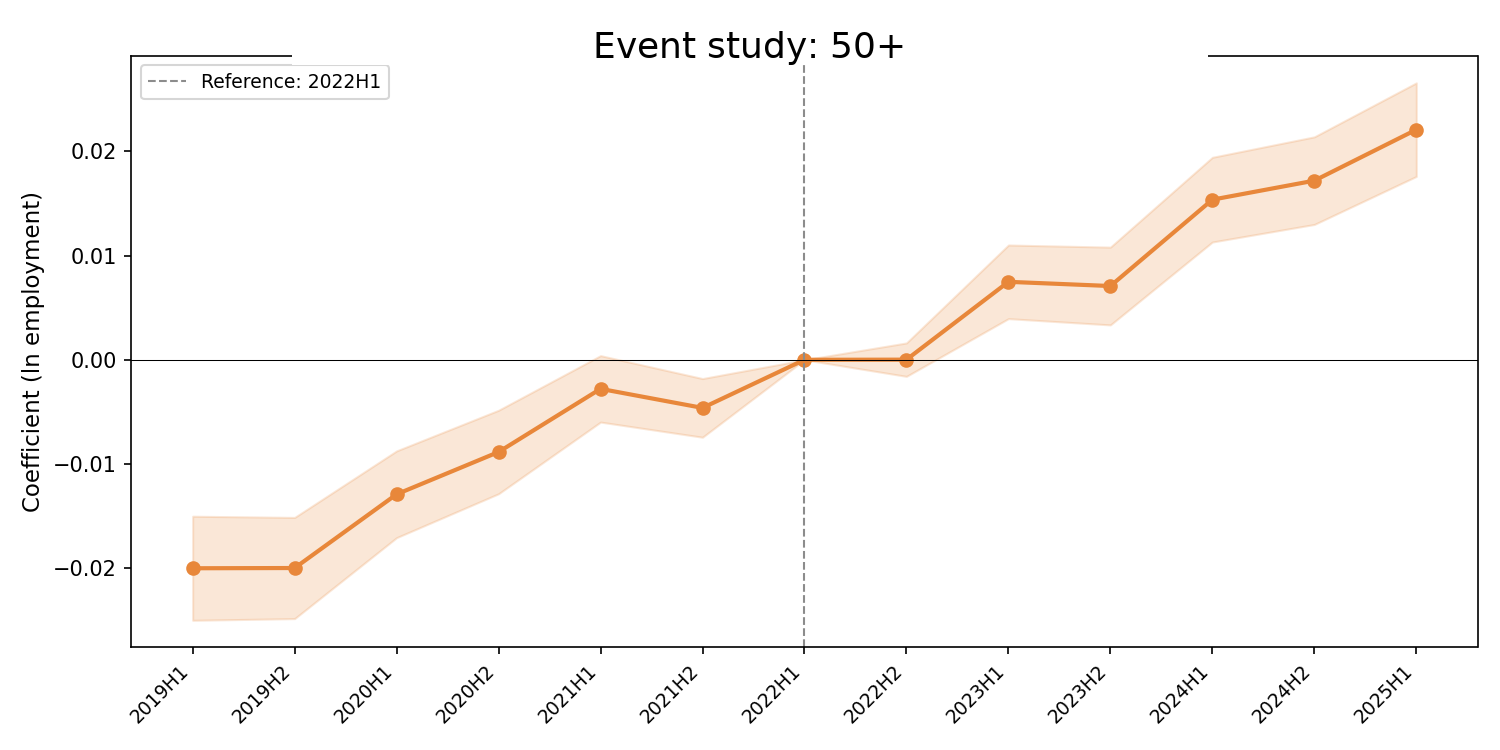
\includegraphics[width=\textwidth]{figA_es_50plus_corrected.png}
\caption{Half-year event study: ages 50+. Employer$\times$quartile and employer$\times$month fixed effects (reference: 2022H1). Significant pre-trends ($\chi^2(6) = 195.7$, $p < 0.001$) reflecting a convergence toward zero. Post-treatment coefficients are positive and rising, consistent with the positive DiD estimate ($+0.015$) for older workers.}
\label{fig:es_50plus}
\end{figure}


\bibliographystyle{elsarticle-harv}
\bibliography{references}

\end{document}
